\chapter{User-Guide\label{chap4:Viertes-Kapitel}}

Im folgenden Kapitel wird ein Überblick über alle implementierten Funktionalitäten aufgezeigt. So dient folgendes Kapitel auch als eine Art \glqq User-Guide\grqq{}.

\section{Login-/Logout-/Nutzerverwaltung\label{sec4.1:Unterpunkt-1}}

\begin{figure}[H]
    \centering
    \begin{minipage}{.4\textwidth}
        \begin{center}
            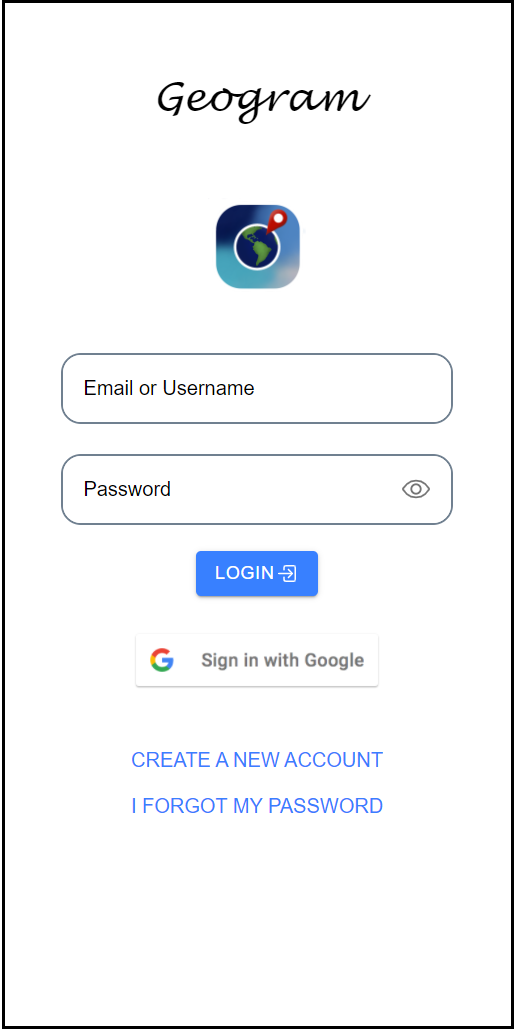
\includegraphics[width=0.8\linewidth]{images/Login.png}
        \end{center}
        \caption{Login - Ansicht}
        \label{fig:login}
    \end{minipage}%
    \begin{minipage}{.6\textwidth}
        \begin{changemargin}{0.5cm}{0cm}            
        Für den Anmeldevorgang benötigt der Besucher ein gültigen Account. Für die eigentliche Anmeldung wird das Passwort mit entweder der E-Mail-Adresse oder dem Usernamen benötigt. Sind die angegebene Anmeldeinformationen nicht korrekt wird dem Besucher ein PopUp mit der Nachricht \glqq \textbf{Your Login credentials are incorrect}\grqq{} angezeigt.

        Neben dem Anmelden kann man über diese Ansicht noch die Funktionalitäten \glqq \textbf{Registrierung}\grqq{} und \glqq \textbf{Password vergessen}\grqq{} aufrufen.
        \end{changemargin}
    \end{minipage}
\end{figure}

\begin{figure}[H]
    \centering
    \begin{minipage}{.4\textwidth}
        \begin{center}
            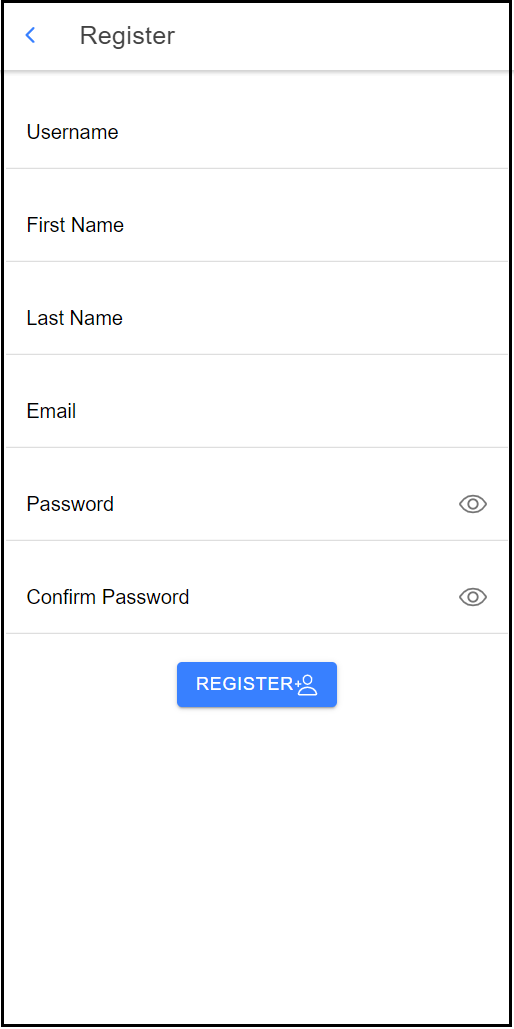
\includegraphics[width=0.8\linewidth]{images/Register.png}
        \end{center}
        \caption{Registrierungs - Ansicht}
        \label{fig:register}
    \end{minipage}%
    \begin{minipage}{.6\textwidth}
        \begin{changemargin}{0.5cm}{0cm}            
            Betätigt man auf der Login-Ansicht den Button \glqq \textbf{CREATE A NEW ACCOUNT}\grqq{}, so gelangt man auf die Registrierungs-Ansicht. Für einen neuen Account benötigt man folgende Informationen:

            \begin{itemize}
                \item \textbf{Username}
                \item \textbf{Vorname}
                \item \textbf{Nachname}
                \item \textbf{E-Mail}
                \item \textbf{Passwort}
            \end{itemize}

            Das Passwort muss folgende Bedingungen erfüllen:
            \begin{itemize}
                \item \textbf{Mindestens 8 Zeichen lang}
                \item \textbf{mind. eine Zahl}
                \item \textbf{mind. ein Sonderzeichen}
            \end{itemize}
        \end{changemargin}
    \end{minipage}
\end{figure}

\begin{figure}[H]
    \centering
    \begin{minipage}{.4\textwidth}
        \begin{center}
            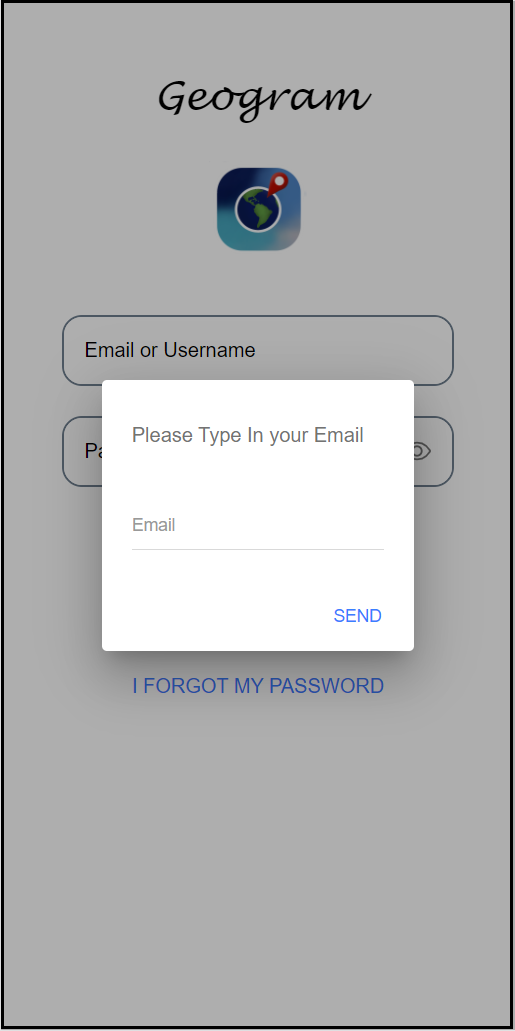
\includegraphics[width=0.8\linewidth]{images/forgetemail.png}
        \end{center}
        \caption{E-Mail-Vergessen - Ansicht}
        \label{fig:forgetemail}
    \end{minipage}%
    \begin{minipage}{.6\textwidth}
        \begin{changemargin}{0.5cm}{0cm}            
            Falls der Besucher sein Password für seinen Account vergessen hat, so kann er mit der \glqq Password-Vergessen\grqq{}-Funktionalität ein neues Password hinterlegen. Hierfür muss er seien gültige Account-E-Mail angeben und erhält von Geogram eine E-Mail zugesendet. In dieser E-Mail befindet sich ein Link, mit welchem der Besucher seinem Account ein neues Password hinterlegen kann.
        \end{changemargin}
    \end{minipage}
\end{figure}

\section{Profil - Ansicht\label{sec4.2:Unterpunkt-2}}

\begin{figure}[H]
    \centering
    \begin{minipage}{.4\textwidth}
        \begin{center}
            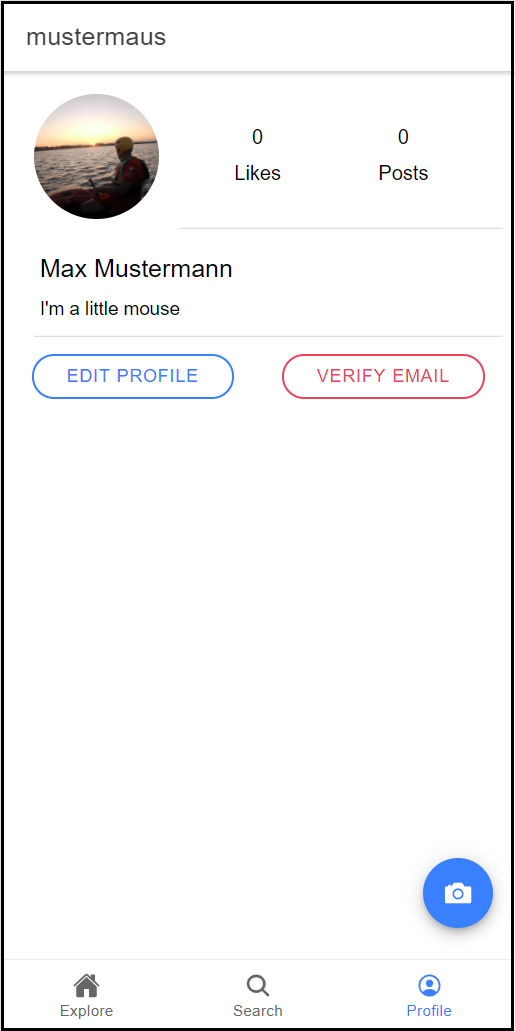
\includegraphics[width=0.8\linewidth]{images/profil.png}
        \end{center}
        \caption{Profil - Ansicht}
        \label{fig:profil}
    \end{minipage}%
    \begin{minipage}{.6\textwidth}
        \begin{changemargin}{0.5cm}{0cm}            
            In der Profil-Ansicht hat der Besucher die Möglichkeit Informationen über sein eigenes Profil zu sehen.

            Zu sehen sind folgende Informationen:
            \begin{itemize}
                \item \textbf{Profilbild}
                \item \textbf{Anzahl erhaltener Likes}
                \item \textbf{Anzahl veröffentlichter Posts}
                \item \textbf{Vor- und Nachname}
                \item \textbf{Biographie (Text über sich selbst)}
            \end{itemize}

            Zusätzlich hat man noch die Möglichkeit folgende Funktionalitäten auf der Profil-Ansicht zu betätigen:
            \begin{itemize}
                \item \textbf{Ändern des Profilbildes (Durch drücken des Bildes)}
                \item \textbf{Profil bearbeiten}
                \item \textbf{Einmalige Verifizierung der E-Mail}
            \end{itemize}
        \end{changemargin}
    \end{minipage}
\end{figure}

\begin{figure}[H]
    \centering
    \begin{minipage}{.4\textwidth}
        \begin{center}
            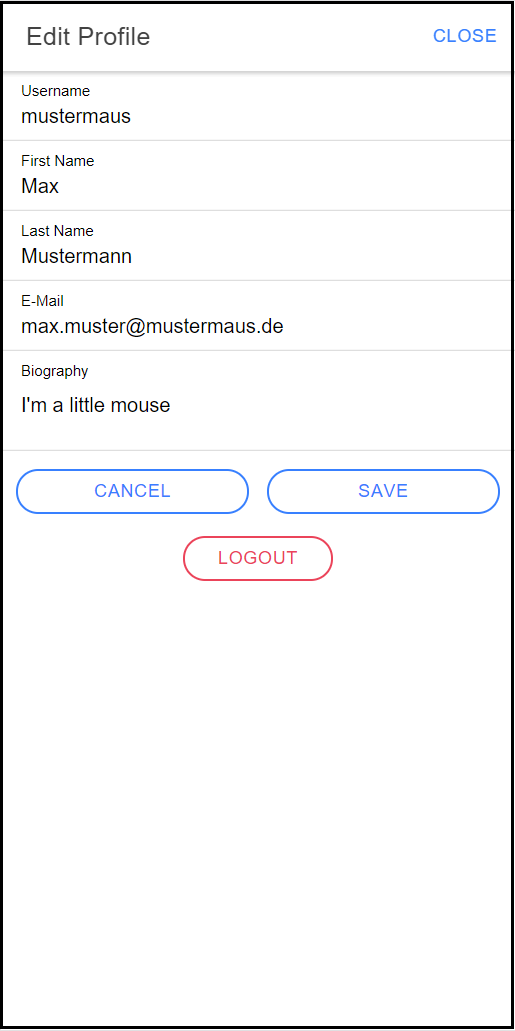
\includegraphics[width=0.8\linewidth]{images/editProfil.png}
        \end{center}
        \caption{Bearbeite Profil - Ansicht}
        \label{fig:editprofil}
    \end{minipage}%
    \begin{minipage}{.6\textwidth}
        \begin{changemargin}{0.5cm}{0cm}            
            In dieser Ansicht hat der Benutzer zusätzlich die Möglichkeit die Informationen des Profils zu überarbeiten.

            Zusätzlich hat man hier die Möglichkeit sich von Geogram abzumelden. Man gelangt dann wieder zur Login-Ansicht.
        \end{changemargin}
    \end{minipage}
\end{figure}
